\documentclass[12pt,letterpaper]{article} 
%\documentclass[12pt,draft]{article}
% Tipo de documento y otras especificaciones
\usepackage[utf8]{inputenc}                   % Para escribir tildes y eñes
\usepackage[spanish]{babel} 
\usepackage{verbatim}
\usepackage{multirow}
\usepackage{bigstrut}
\renewcommand{\labelitemi}{$\bullet$}
\usepackage{pgfgantt}% gantt
% Para que los títulos de figuras, tablas y otros estén en español
\addto\captionsspanish{\renewcommand{\tablename}{Tabla}}					% Cambiar nombre a tablas
\addto\captionsspanish{\renewcommand{\listtablename}{Índice de tablas}}		% Cambiar nombre a lista de tablas
\usepackage{geometry}
\geometry{left=18mm,right=18mm,top=21mm,bottom=21mm} % Tamaño del área de escritura de la página
\usepackage{amsmath}      % Los paquetes ams son desarrollados por la American Mathematical Society
\usepackage{amsfonts}     % y mejoran la escritura de fórmulas y símbolos matemáticos.
\usepackage{amssymb}
\usepackage{graphicx} 
\DeclareGraphicsExtensions{.png,.jpg,.eps,}
% Para insertar gráficas
\usepackage{subfigure}	% Para colocar varias figuras
\usepackage{unitsdef}	  % Para la presentación correcta de unidades
\renewcommand{\unitvaluesep}{\hspace*{4pt}}	% Redimensionamiento del espacio entre magnitud y unidad
\usepackage[colorlinks=true,urlcolor=blue,linkcolor=black,citecolor=black]{hyperref}     % Para insertar hipervínculos y marcadores
\usepackage{float}	 	% Para ubicar las tablas y figuras justo después del texto
\usepackage{booktabs}% Para hacer tablas más estilizadas
\usepackage{adjustbox}
\usepackage{multirow}
\usepackage{mcode}
\usepackage{listings}
\batchmode
\bibliographystyle{plain}
\pagestyle{plain}
\pagenumbering{arabic}
\usepackage{lastpage}
\usepackage{enumerate} 
\usepackage{fancyhdr}	% Para manejar los encabezados y pies de página
\pagestyle{fancy}		% Contenido de los encabezados y pies de pagina
\lhead{IE-0217 Estructuras abstractas de datos y algoritmos para ingeniería} 
\chead{}
\rhead{Proyecto 2}
\lfoot{Escuela de Ingeniería Eléctrica} 
\cfoot{\thepage\ de \pageref{LastPage}}
\rfoot{Universidad de Costa Rica}

\author{Laura Rincón Riveros, B55863\\ Esteban Vargas Vargas, B16998 \\ {\small Grupo 1}\\ Profesor: Ricardo Román \vspace*{1.0in}}
\title{Universidad de Costa Rica\\{\small Facultad de Ingeniería\\Escuela de Ingeniería Eléctrica\\IE-0217 Estructuras abstractas de datos y algoritmos para ingeniería\\II ciclo 2016\\\vspace*{1.5in}} Proyecto 1 \\ Implementación del juego de la vida de Conway  \vspace*{0.7in}}
\date{\today \vspace*{1.0in}}  	
 		
\setcounter{secnumdepth}{5}
%%%%%%%%%%%%%%%%

\usepackage[at]{easylist}
\ListProperties(Style*=,Numbers=a,FinalMark={.})

\Activate
\newcommand{\spobj}{@ } % Explicit space after @ needed!!!!!
\newcommand{\goal}{@@ }
\newcommand{\ind}{@@@ }
\Deactivate

\newenvironment{objectives}
{%
\begin{easylist}
}
{
\end{easylist}
}

\begin{document}	% Inicio del documento
%%%%%%%%%%%%%%%%

\pdfbookmark[1]{Portada}{portada} 	% Marcador para el título

\maketitle							% Título


\newpage
\tableofcontents
\newpage
\listoffigures

\listoftables

\newpage
%%%%%%%%%%%%%%%%%%%%%%%%%%%%%%
\section{Reseña del algoritmo/estructura}
Un \textit{autómata celular} es un modelo matemático que modela un sistema dinámico en pasos discretos. Son redes de autómatas simples que producen una salida a partir de varias entradas, modificando su estado dependiendo de una función de transición. Por lo general, el estado de una célula depende de su estado anterior así como de los estados de las células vecinas. 

Un \textit{autómata celular} tiene las siguientes características:
\begin{itemize}
\item Se compone por una rejilla o espacio celular de \textit{n} celdas.
\item Cada celda puede tomar un estado de entre un número finito de \textit{k} estados.
\item Cada celda tiene una vecindad.
\item Cuenta con una función de transición que define cómo se va a desarrollar la población de células.
\item Su vida se desarrolla en generaciones, es decir, en pasos discretos de tiempo. 
\end{itemize}
En la figura \ref{fig:AM} se muestra un autómata celular.
\begin{figure}[H]
\centering

\includegraphics[width=0.8\textwidth]{img/automataCelular}
\caption{\label{fig:AM} Ejemplo de autómata celular \textit{obtenido de https://app.slidebean.com}}
\end{figure}

El juego de la vida de Conway es un juego-autómata celular propuesto por el matemático británico John Horton Conway en 1970, el cual se hizo popular con su aparición en la revista \textit{Scientific American}. 
Este científico es conocido sobre todo por su teoría de juegos combinatorios, aunque también participó en el desarrollo de teorías como la de números y códigos.\cite{CarlosIII}
El desarrollo de este juego fue motivado por un interés de Conway de explorar y ampliar la teoría de automatas celulares desarrollada por el matemático John Von Neumann en los años 40. 

En el Juego de la Vida, y en general en autómatas celulares, es muy importante el concepto de \textit{vecindad}, ya que esta afecta de manera directa el desarrollo de los estados de todas las células del autómata. Existen dos tipos conocidos: la \textit{vecindad de Moore} y la \textit{vecindad de Von Neumann}. En específico, el Juego de la Vida toma como vecindad de una célula la vecindad de Moore, la cual define que para una célula dada las células vecinas son todas aquellas adyacentes, es decir cada célula tiene una vecindad de 8 semejantes. En contraste la vecindad de von Neumann sólo toma en cuenta las células adyacentes en sentido vertical y horizontal, para un total de cuatro vecinas. En la figura \ref{fig:vecindad} se presentan los conceptos mencionados. 

\begin{figure}[H]
\centering
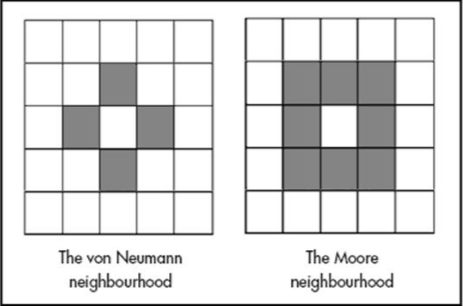
\includegraphics[width=0.75\textwidth]{img/vecindades.png}
\caption{\label{fig:vecindad}Vecindad de von Neumann y de Moore \cite{vec}}
\end{figure}

Luego de su publicación en 1970, el Juego de La Vida atrajo mucha atención ya que era capaz de crear patrones de muy alta complejidad a partir de reglas bastante sencillas.
Otro de los factores que atrajo la atención hacia el Juego de la Vida fue su similitud con procesos evolutivos de poblaciones encontradas en la naturaleza, los cuales también cuentan con generaciones cuyos estados posteriores dependen tanto de su estado actual como del estado de la población a su alrededor. Por estas semejanzas muchos estudiosos de biología, física, matemática e incluso economía y filosofía vieron en el juego potencial para modelar de alguna manera procesos o fenómenos en sus campos.





\newpage 
\section{Funcionamiento del algoritmo/estructura}
El Juego de la Vida es un autómata celular que también se conoce como un juego de 0-jugadores, esto ya que su desarrollo depende solamente de la entrada inicial y no requiere de ninguna intervención externa luego de este paso.

Las células  pueden tener solamente dos estados: viva o muerta. La transición entre estados para cada célula, y por ende la disposición de la población en general, se define una función de transición bastante sencilla, la cual se rige por 4 reglas:
\begin{enumerate}
\item Regla de la soledad: Una célula viva con menos de dos células vivas en su vecindad muere para la siguiente generación.

\begin{figure}[H]
\centering
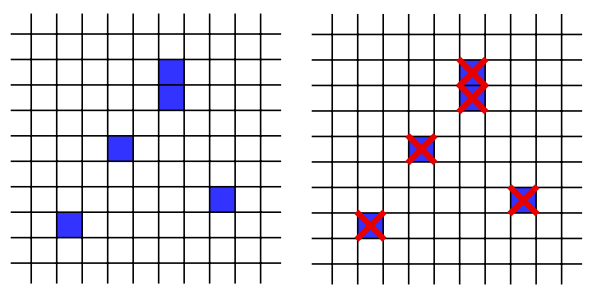
\includegraphics[width=0.75\textwidth]{img/Regla1.png}
\caption{\label{fig:Regla1}Regla 1 Juego de la Vida \cite{Suarez}}
\end{figure}

\item Regla de la supervivencia: Una célula viva con dos o tres células vivas en su vecindad sobrevive para la siguiente generación.

\begin{figure}[H]
\centering
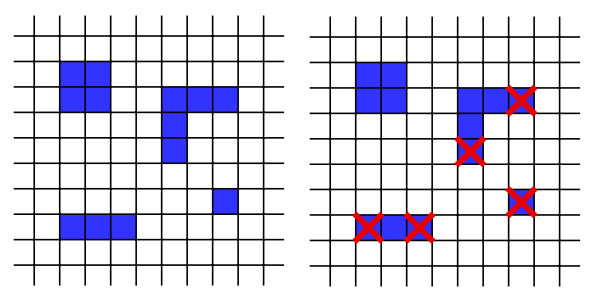
\includegraphics[width=0.75\textwidth]{img/Regla2.png}
\caption{\label{fig:Regla2}Regla 2 Juego de la Vida \cite{Suarez}}
\end{figure}

\item Regla de la sobrepoblación: Una célula viva con más de tres células vivas en su vecindad muere para la siguiente generación.

\begin{figure}[H]
\centering
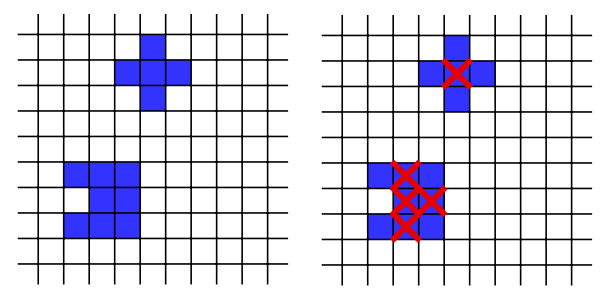
\includegraphics[width=0.75\textwidth]{img/Regla3.png}
\caption{\label{fig:Regla1}Regla 3 Juego de la Vida \cite{Suarez}}
\end{figure}

\item Regla de la reproducción: Una célula muerta con exactamente tres células vivas en su vecindad estará viva para la generación.

\begin{figure}[H]
\centering
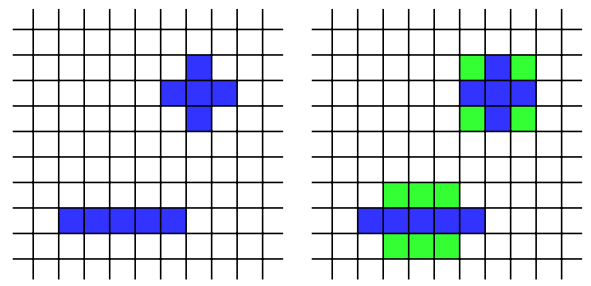
\includegraphics[width=0.75\textwidth]{img/Regla4.png}
\caption{\label{fig:Regla4}Regla 4 Juego de la Vida \cite{Suarez}}
\end{figure}

\end{enumerate}

Dependiendo del patrón inicial, es decir la configuración de células vivas al inicio del juego, se va a ir desarrollando la población siguiendo las reglas antes mencionadas. Su comportamiento se puede clasificar en 3 categorías:

\begin{enumerate}
\item Patrones estáticos: Es una configuración que no produce ni muerte ni renacimiento de células.

\begin{figure}[H]
\centering
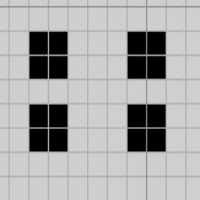
\includegraphics[width=0.4\textwidth]{img/estatico1_.png}
\caption{\label{fig:estatico}Ejemplo de patrón estático \cite{UNAM}}
\end{figure}

\item Patrones oscilantes: Configuración que produce patrones que se repiten a ciertos intervalos de generaciones.

\begin{figure}[H]
\centering
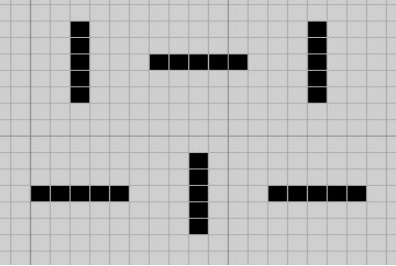
\includegraphics[width=0.4\textwidth]{img/oscilante.png}
\caption{\label{fig:oscilante}Ejemplo de patrón oscilante \cite{UNAM}}
\end{figure}

\item Patrones que se trasladan: Cuando se producen conjuntos de células que se van moviendo por el tablero o rejilla. 

\begin{figure}[H]
\centering

\includegraphics[width=0.5\textwidth]{img/space.png}
\caption{\label{fig:spaceship}Ejemplo de patrón ladeante \cite{UNAM}}
\end{figure}

\end{enumerate}

%\subsection{Metas y entregables}
\newpage 
\section{Objetivos}
\subsection{Objetivo General}
\begin{itemize}
\item Implementar el Juego de la Vida de Conway en C++
\end{itemize}

\subsection{Objetivos específicos}

\begin{objectives}
\begin{itemize}
\item Encontrar la función de tiempo así como la complejidad del algoritmo
\item Verificar que la complejidad es igual para cualquier patrón inicial
\item Comprobar el correcto funcionamiento del programa usando patrones conocidos encontrados en la bibliografía
\end{itemize}

\end{objectives}

\newpage 
\section{Metodología}
\vspace{1em}
En el desarrollo del proyecto sobre la implementación del juego de la vida de Conway, se planteó el procedimiento que se presenta en las siguientes secciones, con el fin de alcanzar los objetivos propuestos.

\subsection{Implementación juego de La vida en C++}

\subsubsection{Funcionamiento del juego de la Vida}
Previo a la realización del algoritmo, fue de gran importancia hacer una búsqueda bibliográfica sobre el funcionamiento del juego de la vida de Conway. Por lo que, se investigó sobre las reglas de supervivencia de células y muerte de células.

Una vez hecha la investigación bibliográfica, se procedió a trabajar en la Estructura del algoritmo.

\subsubsection{Estructura del algoritmo}
Se desarrolló un algoritmo que simulara el juego de la vida en el lenguaje de programación C++. El programa contiene las siguientes funcionalidades:

\begin{itemize}

\item Capacidad de ejecutar cada generación, de un patrón dado, para reproducir la evolución del mismo.
\item Posibilidad de realizar un número específico de generaciones del patrón ingresado.
\item Representar de manera visual el tablero del juego de la vida.

\end{itemize}

A partir de las directrices anteriores, se procedió a crear la estructura del código del programa. Mediante la Programación Orientada a Objeto (POO), se utilizó la siguiente composición: 
\begin{itemize}
\item Clase JuegoDeLaVida: Esta clase tiene los atributos y métodos necesarios para desarrollar la lógica del juego:
\footnote{El signo + se refiere a los atributos y métodos públicos en la Clase JuegoDeLaVida.}
  \begin{itemize}
  \item Atributos:
      \begin{itemize}
      \item [+] dimesionTab: Valor de tipo entero que representa al tamaño (alto y ancho) del tablero, el cuál es cuadrado.
      \item [+] contenidoTab: matriz de valores numéricos que simboliza el patrón de células del juego. Se consideró un 1 como una célula viva y un 0 como una célula muerta.
      \end{itemize}
  \item Métodos:
  	\begin{itemize}
  	\item [+] Iniciar: Encargado de crear una matriz temporal y llamar al método Supervivencia con el patrón inicial. No retorna ningún valor.
    
    Este método tiene una sobrecarga, para permitir ingresar o no el número de generaciones que se quiere obtener.
    \item [+] Supervivencia: Este método contiene las reglas de supervivencia. Por lo cuál, revisa la vencidad de cada una de las células para predecir su estado en la siguiente generación. 
    
    Las generaciones se van construyendo en la matriz temporal, una vez terminado el proceso de comprobación de supervivencia, se iguala la matriz temporal al contenidoTab de la clase. Luego llama al método Imprimir para visualizar la evolución.
   
   Además, es un método sobrecargado para permitir ingresar o no el número de generaciones que se quiere obtener, y no tiene valores de retorno.
   
    \item [+] Vaciar: Método complementario que recorre un tablero y lo vacía, es decir, iguala cada casilla a 0 (célula muerta).
    \item [+] Imprimir: Encargado de recorrer una matriz de entrada e imprimir a manera de tablero su contenido.
  	\end{itemize}
  \end{itemize}
\end{itemize}



\subsection{Representación gráfica}
El programa implementado en C++, imprime a manera de texto el contenido del tablero del juego de la vida. Por lo tanto, se utilizó una biblioteca de Python capaz de recibir una archivo de texto con el contenido de las matrices, para luego crear una imagen con determinado número de pixeles. 

Con ayuda de la biblioteca Pillow se construyó una imagen para cada generación de célular y adicionamente se utilizó Microsoft PowerPoint para observar de manera dinámica la secuencia de las imágenes.

\subsection{Tiempos de ejecución y complejidad computacional}
Para obtener la función del tiempo de ejecución y la complejidad computacional fue necesario emplear el Teorema Maestro. Se utilizó la Tabla \ref{tabtiempo} para designar los valores en unidades de tiempo a los instructivos.

\begin{table}[H]
\centering
\caption{Valor por unidad de tiempo de los instructivos del programa.}
\label{tabtiempo}
\begin{tabular}{|c|l|}
\hline 
\textbf{Valor en unidad de tiempo} & \multicolumn{1}{c|}{\textbf{Comando}}                \\ \hline
1                                  & Asignación e inicialización                                                  \\ \hline
1                                  & Llamado a memoria                                                            \\ \hline
1                                  & Operaciones de suma o resta                          \\ \hline
1                                  & Comparación                                                                  \\ \hline
1                                  & Función cout                                                               \\ \hline
1*c                                & If(c), donde c es el número de comparaciones                                 \\ \hline
i*n                                & for(), n son las veces que se repite e i son las intrucciones dentro del for \\ \hline
\end{tabular}
\end{table}


De esta manera, se contabilizó las líneas de comando necesarias para la ejecución del programa y se calculó teóricamente la función de Tiempo. 

Posteriormente, se utilizó la biblioteca Time.h para medir experimentalemente el tiempo que requería el algoritmo para su ejecución con el fin de comparar la función teórica con los resultados experimentales. Para las pruebas experimentales se utilizó una computadora Dell con sistema operativo Ubuntu 14.04, Intel(R) Core(TM)  i3- 3277U CPU con 1.9GHz. 

Con el debido análisis de la función de Tiempo, se procedió a establecer la complejidad del algoritmo implementado.


\newpage
\section{Resultados}
A continuación se presentan los resultados obtenidos con el proyecto sobre la implementación del juego de la vida de Conway. Se presentarán en secciones acorde con la metodología para su mejor comprensión.

\subsection{Implementación Juego de La vida en C++}
Se elaboró una Clase JuegoDeLaVida con la estructura mostrada en la Figura \ref{UML}.\footnote{El signo + se refiere a los atributos y métodos públicos en la Clase JuegoDeLaVida.} 

\begin{figure}[H]
\centering
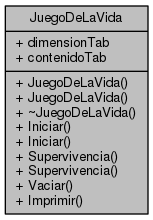
\includegraphics[height=10 cm, width=7cm]{img/UML}
\caption{\label{UML} Diagrama de la clase JuegoDeLaVida, generado por Doxygen}
\end{figure}
\footnote{Se puede disponer del Código fuente en la sección de Anexos.}
Con el objetivo de comprobar la funcionalidad del código, se ejecutaron varios patrones para asegurar que estuvieran evolucionando acorde las reglas del juego. A continuación se presenta un ejemplo de patrón, con matrices de 1 y 0. El código se implementó de tal manera que la salida, es decir la matriz de 1's y 0's se imprimiera tanto en consola como en un archivo de texto out.txt; el cual sería posteriormente leído por el programa de Python para crear las imágenes de cada generación. 

\begin{figure}[H]
\centering
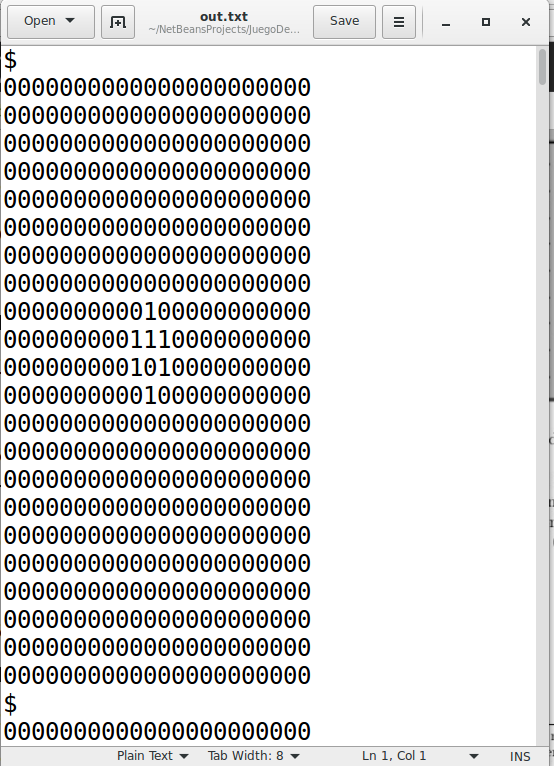
\includegraphics[height=12 cm, width=12cm]{img/outtxt.png}
\caption{\label{outtxt} Out.txt}
\end{figure}


%%%%%%%%%%%%%%%%%%%%%%%%%%%%%%%%%% Imagenes ¡¡¡¡ESTEBAN!!!!! %%%%%%%%%%%%%%%%%%%
\newpage 
\subsection{Representación gráfica mediante uso de Python}
Para poder representar la salida del programa de una manera gráfica se procedió a crear un código en Python utilizando la biblioteca \textit{Pillow}. A partir del archivo out.txt mostrado en la sección anterior, se crearon imágenes pixel por pixel para cada generación. Esto se logró dividiendo en impresión cada generación mediante un símbolo $\$$. 

Al tener una imágen para cada generación se procedió a hacerles una modificación de tamaño y luego mediante la herramienta de Microsoft Powerpoint se creó un video para unir las imágenes. En la figura \ref{video} se muestra por ejemplo la cuarta generación del patrón \textit{10-cell-row}.

\begin{figure}[H]
\centering

\includegraphics[height=12 cm, width=15cm]{img/Ejemplo10cellrow.png}
\caption{\label{video} Cuarta generación 10-cell-row}
\end{figure}

\newpage 
\subsection{Tiempos de ejecución y complejidad computacional}

\subsubsection{Teórico}
Se utilizó la Tabla \ref{tabtiempo} para obtener la función de tiempo\footnote{Revisar el archivo JuegoDeLaVida.txt}, lo cuál resultó en dos funciones de tiempo debído a la sobrecarga de métodos: 

\begin{equation}
T_{1}(n,p)= 208 144n^2 + 20n + 24 + p
\end{equation}

\begin{equation}
T_{2}(N,n,p)= 600Nn^2 + 224n^(2) - 1200Nn + 600N + 20n + 22 + p
\end{equation}
En las cuales, n se refiere a la dimensión del tablero (dimensionTab), N al número de generaciones y p al tiempo que requiere la construcción del patron inicial.

\subsubsection{Experimental}
Para verificar experimentalmente la función de Tiempo se utilizó la ecuación (2), en la cuál se estableción una valor constante de N=10 generaciones y el siguiente patrón inicial:


\begin{figure}[H]
\centering

\includegraphics[height= 5cm, width= 5cm]{img/blinker}
\caption{\label{blinker} Blinker, patrón inicial en las pruebas de tiempo.\textit{Obtenido de http://www.mdpi.com/1424-8220/12/8/10990/htm}}
\end{figure}

Los resultados del tiempo para dicho patrón se presentan en la tabla \ref{pruebastiempo}.
Como complemento se expone las gráficas respectivas de la función de tiempo teórico y experimental.

\begin{table}[H]

\caption{Datos obtenidos al realizar las pruebas de tiempo en Blinker con N=10.}
\label{pruebastiempo}
\centering
\begin{adjustbox}{max width=\textwidth, height= 1.6cm}
\begin{tabular}{|c|c|c|c|c|c|c|c|c|c|c|c|c|}
\hline
\textbf{\begin{tabular}[c]{@{}c@{}}Tamaño \\ (N)\end{tabular}} & \textbf{\begin{tabular}[c]{@{}c@{}}Tiempo \\ Teórico (u.t)\end{tabular}} & \textbf{\begin{tabular}[c]{@{}c@{}}t1 \\ exp\end{tabular}} & \textbf{\begin{tabular}[c]{@{}c@{}}t2 \\ exp\end{tabular}} & \textbf{\begin{tabular}[c]{@{}c@{}}t3 \\ exp\end{tabular}} & \textbf{\begin{tabular}[c]{@{}c@{}}t4 \\ exp\end{tabular}} & \textbf{\begin{tabular}[c]{@{}c@{}}t5 \\ exp\end{tabular}} & \textbf{\begin{tabular}[c]{@{}c@{}}t6 \\ exp\end{tabular}} & \textbf{\begin{tabular}[c]{@{}c@{}}t7 \\ exp\end{tabular}} & \textbf{\begin{tabular}[c]{@{}c@{}}t8 \\ exp\end{tabular}} & \textbf{\begin{tabular}[c]{@{}c@{}}t9 \\ exp\end{tabular}} & \textbf{\begin{tabular}[c]{@{}c@{}}t10 \\ exp\end{tabular}} & \textbf{\begin{tabular}[c]{@{}c@{}}Tiempo \\ experimental \\ promedio (ms)\end{tabular}} \\ \hline
\textbf{50}                                                    & 14 963 826                                                               & 8.719                                                      & 4.738                                                      & 5.199                                                      & 6.166                                                      & 4.997                                                      & 6.268                                                      & 4.695                                                      & 4.631                                                      & 6.268                                                      & 4.633                                                       & 4.541                                                                                    \\ \hline
\textbf{100}                                                   & 61 042 022                                                               & 25.116                                                     & 30.539                                                     & 39.447                                                     & 24.998                                                     & 22.708                                                     & 39.028                                                     & 38.028                                                     & 28.471                                                     & 27.598                                                     & 23.956                                                      & 22.058                                                                                   \\ \hline
\textbf{200}                                                   & 246 564 022                                                              & 132.204                                                    & 162.203                                                    & 109.26                                                     & 149.089                                                    & 160.346                                                    & 100.789                                                    & 130.622                                                    & 187.272                                                    & 156.236                                                    & 149.566                                                     & 113.163                                                                                  \\ \hline
\textbf{400}                                                   & 991 048 022                                                              & 445.545                                                    & 446.208                                                    & 475.934                                                    & 517.128                                                    & 414.688                                                    & 573.638                                                    & 441.245                                                    & 514.166                                                    & 483.623                                                    & 507.464                                                     & 486.010                                                                                  \\ \hline
\textbf{800}                                                   & 3 973 782 022                                                            & 1611.9                                                     & 1586.6                                                     & 1625.5                                                     & 1603.8                                                     & 1684.7                                                     & 1613.7                                                     & 1599.9                                                     & 1647.3                                                     & 1688.2                                                     & 1697.4                                                      & 1635.9                                                                                   \\ \hline
\end{tabular}
\end{adjustbox}
\end{table}

\begin{figure}[H]
\centering
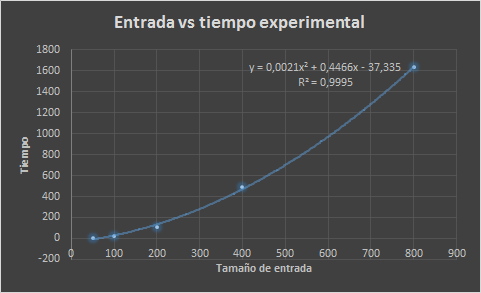
\includegraphics[height= 10cm, width=\textwidth]{img/grafica1}
\caption{\label{Texp} Gráfico de Función de Tiempo experimental}
\end{figure}

\begin{figure}[H]
\centering
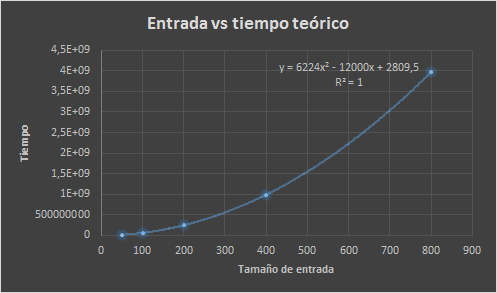
\includegraphics[height= 10cm, width=\textwidth]{img/grafica2}
\caption{\label{Tteo} Gráfico de Función de Tiempo teórico}
\end{figure}

Los resultados obtenidos con la función de tiempo, muestran que el programa posee una complejidad computacional dada por la ecuación (3).

\begin{equation}
\Theta(n)= n^{2}
\end{equation}

\newpage 
\section{Análisis de tiempos de ejecución y complejidad computacional}
En la función de tiempo de ejecución se obtuvo dos ecuaciones debido a la sobrecarga de métodos. Sin embargo, la ecuación (1) es una caso singular de cuando N=100; por lo que utilizó la ecuación (2) donde N puede adquirir un valor mayor a 100.


Al conseguir los resultados de la prueba experimental, dados en la Tabla \ref{tabtiempo}, se puede notar que ambas funciones contienen pendientes bastante distintas que pueden deberse a factores externos del código. No obstante, hay que rescatar que forma carística de las funciones, en la Figura \ref{Tteo} y Figura \ref{Texp} se puede notar una función polinómica de grado 2. Con lo cuál, se puede analizar que la función teórica acota superiormente a la función experimental.


Dado que ambas gráficas son consistentes con su forma, se concluye que debía a su comportamiento ante una entrada, el programa posee una complejidad computacional dada por la ecuación (3), que también se puede deducir de la función de Tiempo de la ecuación (2), para un valor dado de N y p.


Esta compejidad se mantiene indiferentemente del patrón ingresado, debido a que la dimensión del tablero siempre se mantiene igual. Los distintos patrones sólo provocan unas cuantas asignaciones más o menos de 1's a la matriz, las cuales tienen función de tiempo 1, por lo que su efecto en la función de tiempo es bastante despreciable y por ende, la variable \textit{P} no tiene efecto en la complejidad del algoritmo.

\newpage 
\section{Conclusiones}
\begin{itemize}
\item Se implementó de manera satisfactoria el Juego de la Vida de Conway en C++.
\item Se encontró la función de tiempo teórica y se comprobó mediante expermientos.
\item La complejidad del algoritmo de interés es polinómica de grado 2.
\item La complejidad algorítmica del juego de la vida no depende del patrón inicial.
\item Los patrones ingresados en el juego elaborado se comportaron de la manera esperada.
\end{itemize}

\newpage 
\begin{thebibliography}{1}

\bibitem{1} Castillo.J y Rubio.G. (2008).\textit{Trabajo de Bioinformática. Universidad de Castilla-La Mancha}.Obtenido de https://www.dsi.uclm.es/personal/MiguelFGraciani/mikicurri/Docencia/Bioinformatica/web$\_$BIO/Documentacion/Trabajos/El$\%20$juego$\%20$de$\%20$la$\%20$vida$\%20$de$\%20$Conway/Memoria.pdf el martes 4 de octubre del 2016.

\bibitem{CarlosIII}Romero.M (S.F). \textit{El juego de la vida. [Inteligencia en redes de comunicaciones]}. Universidad Carlos III de Madrid, España. Obtenido de http://www.it.uc3m.es/jvillena/irc/practicas/09-10/04mem.pdf el martes 4 de octubre del 2016.

\bibitem{UNAM}López,A. (2011). \textit{Introducción a la vida artificial y autómatas celulares}. Facultad de estudios superiores UNAM, México. Obtenido de http://uncomp.uwe.ac.uk/genaro/Papers/Veranos$\_$McIntosh$\_$files/vida$\_$artificial$\_$Miriam.pdf el martes 4 de octubre del 2016.

\bibitem{Suarez}Suarez, M. (2011). \textit{Autómatas celulares}. Facultad de Ciencias Exactas y Naturales Universidad de Buenas Aires, Argentina. Obtenido de http://cms.dm.uba.ar/actividades/semana/2011/charla.pdf el martes 4 de octubre del 2016.

\bibitem{vec} Tomado de la presentación \textit{Modelos basados en agentes} disponible en http://slideplayer.es/slide/1846954/.
\end{thebibliography}


\newpage

\section{Anexos}

\subsection{Código fuente del Juego de la Vida en C++}
A continuación se muestran los archivos realizados para la implementación del Juego de la Vida de Conway.
\subsubsection{JuegoDeLaVida.h}
\lstset {language=C}
\begin{lstlisting}
#ifndef JUEGODELAVIDA_H
#define JUEGODELAVIDA_H
#include <iostream>

class JuegoDeLaVida{
public:
	
    /*Constructor vacio de JuegoDeLaVida*/
    JuegoDeLaVida();
    
    JuegoDeLaVida(int dimensionTab, int** contenidoTab);
    
    virtual ~JuegoDeLaVida();
    
    /*Atributos de JuegoDeLaVida*/
    int dimensionTab;
    int** contenidoTab;
    
    /*Funciones de JuegoDeLaVida*/
    void Iniciar(JuegoDeLaVida&);
    void Iniciar(JuegoDeLaVida&,int NumGen);
    void Supervivencia(JuegoDeLaVida&,int** contTemporal);
    void Supervivencia(JuegoDeLaVida&,int** contTemporal, int NumGen);
    void Vaciar(JuegoDeLaVida&);
    void Imprimir(const JuegoDeLaVida&);

}; #endif /* JUEGODELAVIDA_H */

\end{lstlisting}
\subsubsection{JuegoDeLaVida.cpp}
\lstset {language=C}
\begin{lstlisting}
#include "JuegoDeLaVida.h"
using namespace std;

///Constructor vacio de JuegoDeLaVida
JuegoDeLaVida::JuegoDeLaVida(){
    
}

///Constructor de JuegoDeLaVida
JuegoDeLaVida::JuegoDeLaVida(int dimensionTab, int** contenidoTab){
    this->dimensionTab = dimensionTab;
    this->contenidoTab = contenidoTab;
}

///Destructor de JuegoDeLaVida
JuegoDeLaVida::~JuegoDeLaVida(){
}

void JuegoDeLaVida::Iniciar(JuegoDeLaVida&){
    ///////////////////////////////////////////
    
    ///Construccion arreglo 2d para el Tablero temporal
    int** contTemporal = new int*[dimensionTab];
    for (int i = 0; i < dimensionTab; i++) {
        contTemporal[i] = new int[dimensionTab];
    }
    ///Inicializacion valores Tablero temporal
    for (int i = 0; i < dimensionTab; i++) {
        for (int j = 0; j < dimensionTab; j++) {
            contTemporal[i][j] = 0;
        }
    }
    /////////////////////////////////////////////
    
    JuegoDeLaVida* Jtemp = new JuegoDeLaVida(this->dimensionTab,this->contenidoTab);
    Jtemp->Supervivencia(*Jtemp,contTemporal);
}

void JuegoDeLaVida::Iniciar(JuegoDeLaVida&, int NumGen){
    ///////////////////////////////////////////
    
    ///Construccion arreglo 2d para el Tablero temporal
    int** contTemporal = new int*[dimensionTab];
    for (int i = 0; i < dimensionTab; i++) {
        contTemporal[i] = new int[dimensionTab];
    }
    ///Inicializacion valores Tablero temporal
    for (int i = 0; i < dimensionTab; i++) {
        for (int j = 0; j < dimensionTab; j++) {
            contTemporal[i][j] = 0;
        }
    }
    /////////////////////////////////////////////
    
    JuegoDeLaVida* Jtemp = new JuegoDeLaVida(this->dimensionTab,this->contenidoTab);
    Jtemp->Supervivencia(*Jtemp,contTemporal,NumGen);
    ofstream myfile ("out.txt", ios::app);
    myfile<< "@"<<endl;
    myfile.close();
    
}

void JuegoDeLaVida::Supervivencia(JuegoDeLaVida&,int** contTemporal, int NumGen){
    JuegoDeLaVida* Jtemp = new JuegoDeLaVida(this->dimensionTab,this->contenidoTab);
    for(int a=0;a<NumGen;a++){
        for (int i = 1; i < dimensionTab-1; i++) {
            for (int j = 1; j < dimensionTab-1; j++) {
                ///Renacimiento celulas 
                if(contenidoTab[i][j] == 0){
                    int temp1=0;
                    if(contenidoTab[i][j-1]==1){temp1++;}
                    if(contenidoTab[i][j+1]==1){temp1++;}
                    if(contenidoTab[i-1][j-1]==1){temp1++;}
                    if(contenidoTab[i-1][j]==1){temp1++;}
                    if(contenidoTab[i-1][j+1]==1){temp1++;}
                    if(contenidoTab[i+1][j-1]==1){temp1++;}
                    if(contenidoTab[i+1][j]==1){temp1++;}
                    if(contenidoTab[i+1][j+1]==1){temp1++;}
                    //cout<<"i="<<i<<" j="<<j<<" temp1="<<temp1<<endl;
                    if(temp1==3){contTemporal[i][j]=1;}
                    if(temp1<3 || temp1>3){contTemporal[i][j]=0;}

                }
                ///Supervivencia celulas
                else if(contenidoTab[i][j] == 1){
                    int temp2=0;
                    if(contenidoTab[i][j-1]==1){temp2++;}
                    if(contenidoTab[i][j+1]==1){temp2++;}
                    if(contenidoTab[i-1][j-1]==1){temp2++;}
                    if(contenidoTab[i-1][j]==1){temp2++;}
                    if(contenidoTab[i-1][j+1]==1){temp2++;}
                    if(contenidoTab[i+1][j-1]==1){temp2++;}
                    if(contenidoTab[i+1][j]==1){temp2++;}
                    if(contenidoTab[i+1][j+1]==1){temp2++;}
                    //cout<<"i="<<i<<" j="<<j<<" temp2="<<temp2<<endl;
                    if(temp2==2 || temp2==3){contTemporal[i][j]=1;}
                    if(temp2<2 || temp2>3){contTemporal[i][j]=0;}

                }
            }
        }
        ///Igualacion contenido a contenido temporal
        for (int i = 0; i < dimensionTab; i++) {
            for (int j = 0; j < dimensionTab; j++) {
                contenidoTab[i][j] = contTemporal[i][j];
            }
        }
        
        Jtemp->Imprimir(*Jtemp);
	}
}

void JuegoDeLaVida::Supervivencia(JuegoDeLaVida&,int** contTemporal){
    JuegoDeLaVida* Jtemp = new JuegoDeLaVida(this->dimensionTab,this->contenidoTab);
    while(contenidoTab!= contTemporal){
        for (int i = 1; i < dimensionTab-1; i++) {
            for (int j = 1; j < dimensionTab-1; j++) {
                ///Renacimiento celulas 
                if(contenidoTab[i][j] == 0){
                    int temp1=0;
                    if(contenidoTab[i][j-1]==1){temp1++;}
                    if(contenidoTab[i][j+1]==1){temp1++;}
                    if(contenidoTab[i-1][j-1]==1){temp1++;}
                    if(contenidoTab[i-1][j]==1){temp1++;}
                    if(contenidoTab[i-1][j+1]==1){temp1++;}
                    if(contenidoTab[i+1][j-1]==1){temp1++;}
                    if(contenidoTab[i+1][j]==1){temp1++;}
                    if(contenidoTab[i+1][j+1]==1){temp1++;}
                    //cout<<"i="<<i<<" j="<<j<<" temp1="<<temp1<<endl;
                    if(temp1==3){contTemporal[i][j]=1;}
                    if(temp1<3 || temp1>3){contTemporal[i][j]=0;}

                }
                ///Supervivencia celulas
                else if(contenidoTab[i][j] == 1){
                    int temp2=0;
                    if(contenidoTab[i][j-1]==1){temp2++;}
                    if(contenidoTab[i][j+1]==1){temp2++;}
                    if(contenidoTab[i-1][j-1]==1){temp2++;}
                    if(contenidoTab[i-1][j]==1){temp2++;}
                    if(contenidoTab[i-1][j+1]==1){temp2++;}
                    if(contenidoTab[i+1][j-1]==1){temp2++;}
                    if(contenidoTab[i+1][j]==1){temp2++;}
                    if(contenidoTab[i+1][j+1]==1){temp2++;}
                    //cout<<"i="<<i<<" j="<<j<<" temp2="<<temp2<<endl;
                    if(temp2==2 || temp2==3){contTemporal[i][j]=1;}
                    if(temp2<2 || temp2>3){contTemporal[i][j]=0;}

                }
            }
        }
        ///Igualacion contenido a contenido temporal
        for (int i = 0; i < dimensionTab; i++) {
            for (int j = 0; j < dimensionTab; j++) {
                contenidoTab[i][j] = contTemporal[i][j];
            }
        }
        
        Jtemp->Imprimir(*Jtemp); 
    }
    
}

void JuegoDeLaVida::Imprimir(const JuegoDeLaVida&){
    ofstream myfile ("out.txt", ios::app);//**NUEVO**
    myfile<< "$"<<endl;//**NUEVO**
    for(int i = 0; i < dimensionTab; i++){
        for(int j=0; j< dimensionTab ;j++){
            cout << contenidoTab[i][j] << " ";
            myfile << contenidoTab[i][j];
            }
        cout << endl;
        myfile<< endl;
    }
    myfile.close();
    cout<<"------------------------"<<endl;
}

void JuegoDeLaVida::Vaciar(JuegoDeLaVida&){
    for(int i = 0; i < dimensionTab; i++){
        for(int j=0; j< dimensionTab ;j++){
            contenidoTab[i][j]=0;
        }
    }
}

\end{lstlisting}
\subsubsection{main.cpp}
\lstset {language=C}
\begin{lstlisting}
#include "JuegoDeLaVida.h"
using namespace std;
int main(int argc, char *argv[]) {
    
    cout << "Juego de la vida" << endl << "-----------------------" << endl;
    ///Construccion arreglo 2d para el tablero
    int dimension=22;
    int** cont = new int*[dimension];
    for (int i = 0; i < dimension; i++) {
        cont[i] = new int[dimension];
    }
    
    ///Inicializacion valores tablero valores Tablero
    for (int i = 0; i < dimension; i++) {
        for (int j = 0; j < dimension; j++) {
            cont[i][j] = 0;
        }
    }
    //*******************************************************//
    ///Construccion patrones
    ///Patron bloques centrales oscilantes
//    cont[3][3]=1;
//    cont[3][4]=1;
//    cont[4][3]=1;
//    cont[4][4]=1;
//    
//    cont[5][5]=1;
//    cont[5][6]=1;
//    cont[6][5]=1;
//    cont[6][6]=1;
    
    ///Patron linea oscilante vertical-horizontal
//    cont[5][4]=1;
//    cont[5][5]=1;
//    cont[5][6]=1;
    
    //Patron "small exploder"
    cont[8][10]=1;
    cont[9][9]=1;
    cont[9][10]=1;
    cont[9][11]=1;
    cont[10][9]=1;
    cont[10][11]=1;
    cont[11][10]=1;
    
    //Patron "10-cell row"
//    for(int i = 5 ; i < 15 ; i ++){
//    cont[10][i]=1;
//    }
    
    
    ///Construccion e impresion estado inicial tablero
    
    cout <<"******Patron inicial*****"<<endl;
    JuegoDeLaVida* J1=new JuegoDeLaVida(dimension,cont);
    J1->Imprimir(*J1);
    cout <<"************************"<<endl;

    /////////////////////////////////////////////
    
    J1->Iniciar(*J1,20);
     
    cout<<"-----------------------"<<endl;
    return 0;
}

\end{lstlisting}
\subsection{Código fuente de creación de imágenes en Python}
\begin{lstlisting}
from PIL import Image, ImageDraw
import sys
#ejemplo de ejecucion: python a.py a.csv 500 500

#reader = open('~/NetBeansProjects/JuegoDeLaVida/out.txt',"r")
maxRow=int(sys.argv[2])
maxCol=int(sys.argv[3])
with open(sys.argv[1], 'r') as f:
	a=f.readline().strip()
	b=0
	c=0	
	while a !='@':
		if(a=='$'):
			c+=1
			out = Image.new("L",(int(sys.argv[2]),int(sys.argv[3])))#no tocar
			dout = ImageDraw.Draw(out)#salida que crea una imagen
			a=f.readline().strip()
			for i in range(0,maxRow):
				for j in range(0,maxCol):
					if(a[j]=="1"):
						dout.point((j,i),0)#pixel 0 y 1 pintar de color 2
					else:
						dout.point((j,i),255)#pixel 0 y 1 pintar de color 2
				a=f.readline().strip()
				out.save("out"+ str(c)+".png" , "PNG")

\end{lstlisting}
%%%%%%%%%%%%%%
\end{document}
%%%%%%%%%%%%%% 